\documentclass[aspectratio=169,11pt]{beamer}

\usepackage{amsmath}
\usepackage{array}
\usepackage{booktabs}
\usepackage{graphicx}
\usepackage{siunitx}
\usepackage{xcolor}
\usepackage{xurl}

\usetheme{Madrid}
\usecolortheme{default}
\setbeamertemplate{navigation symbols}{}
\setbeamertemplate{footline}[frame number]
\graphicspath{{assets/}}
\urlstyle{same}

\definecolor{goodGreen}{RGB}{35,120,75}
\definecolor{warnRed}{RGB}{170,55,55}
\definecolor{aaltoBlue}{RGB}{0,83,155}

\newcommand{\good}[1]{\textcolor{goodGreen}{#1}}
\newcommand{\warn}[1]{\textcolor{warnRed}{#1}}
\newcommand{\blue}[1]{\textcolor{aaltoBlue}{#1}}
\newcommand{\src}[1]{\vfill{\tiny\textcolor{gray!70!black}{Source: \url{#1}}}}
\newcommand{\pathtext}[1]{{\scriptsize\url{#1}}}
\newcolumntype{L}[1]{>{\raggedright\arraybackslash}p{#1}}
\newcolumntype{R}[1]{>{\raggedleft\arraybackslash}p{#1}}

\title[Baseline Comparison]{Physics Baselines, Production MLP, and SVGP}
\subtitle{2026-05-21 full-clean / uncensored CDF / P50--Q1 evaluation}
\author{Linan Jiang}
\institute{Aalto University}
\date{21 May 2026}

\begin{document}

\begin{frame}
  \titlepage
\end{frame}

\begin{frame}{Why This Deck Was Refreshed}
\small
\begin{block}{Old version}
The earlier baseline deck described an early-May intermediate model and a
narrative centered on improvement over an early GP baseline.
\end{block}

\begin{block}{Current thesis protocol}
The updated comparison uses the 2026-05-21 evaluation artifacts: production
MLP five seeds, the mu-anchor/raw-uncertain variant, Stage-3 SVGP, and refreshed
Hiroyasu--Arai / Naber--Siebers curve baselines.
\end{block}

\begin{block}{One-line result}
\good{The production MLP strongly beats HA/NS physics baselines. SVGP remains
slightly better on point RMSE/MAE. The MLP is the more conservative uncertainty
surrogate for screening.}
\end{block}
\end{frame}

\begin{frame}{Evaluation Contract}
\small
\begin{tabular}{L{0.26\linewidth}R{0.17\linewidth}R{0.18\linewidth}L{0.31\linewidth}}
\toprule
Protocol & Points & Conditions / trajectories & Role \\
\midrule
Full-clean CDF & \num{692942} & \num{24316} trajectories & Main headline comparison on the common clean CDF set. \\
Conservative uncensored CDF & \num{542565} & 592 conditions & Removes conservatively flagged FOV right-censoring and signal-decay time bins. \\
P50 observed & \num{4213} & 495 conditions & Condition-level P50 observed target for robust mean-head checks. \\
Q1 extrapolated grid & \num{21527} & 495 conditions & P50/Q1 fit grid for extrapolated lower-quantile behavior. \\
\bottomrule
\end{tabular}

\vspace{0.6em}
\footnotesize
The protocols answer different questions: full-clean CDF measures overall point
accuracy, uncensored CDF controls censoring bias, and P50/Q1 checks condition-level
robustness and extrapolation.
\src{Thesis/generated/baseline_comparison_20260521/summary.json}
\end{frame}

\begin{frame}{Models Compared}
\small
\begin{tabular}{L{0.30\linewidth}L{0.58\linewidth}}
\toprule
Model & Setup \\
\midrule
Hiroyasu--Arai calibrated & Empirical curve baseline recalibrated under the current clean protocol. \\
Naber--Siebers delay & Empirical curve baseline with delay handling, also refit. \\
Production MLP & Stage-3 \texttt{anchor\_off}, seeds 7/17/42/99/2024, reported as mean \(\pm\) std. \\
mu-anchor raw-uncertain prodKD & Same data and teacher warm start, but with the mu-anchor/raw-uncertain/product-KD variant. \\
Stage-3 SVGP & Sparse heteroscedastic GP baseline, seed 42, evaluated on the same tables. \\
\bottomrule
\end{tabular}

\vspace{0.7em}
\begin{block}{Boundary}
\footnotesize
This is a same-data evaluation comparison, not a LONO comparison. LONO remains a
separate generalization stress test in the stage-1/2/3 ablation decks.
\end{block}
\end{frame}

\begin{frame}{Full-Clean Headline}
\scriptsize
\begin{tabular}{L{0.29\linewidth}R{0.10\linewidth}R{0.10\linewidth}R{0.10\linewidth}R{0.10\linewidth}R{0.10\linewidth}R{0.10\linewidth}}
\toprule
Model & RMSE & MAE & Bias & P95 & Cov1 & Cov2 \\
\midrule
Hiroyasu--Arai & 11.268 & 8.658 & +0.288 & 22.891 & 0.615 & 0.912 \\
Naber--Siebers & 10.545 & 8.177 & -0.442 & 21.253 & 0.637 & 0.919 \\
\good{Production MLP mean(5)} & \good{4.735} & \good{3.293} & +0.626 & \good{9.167} & \good{0.867} & \good{0.985} \\
mu-anchor raw-uncertain & 5.200 & 3.654 & -0.585 & 10.525 & 0.834 & 0.985 \\
\blue{SVGP Stage-3} & \blue{4.628} & \blue{3.173} & -0.070 & 9.242 & 0.703 & 0.939 \\
\bottomrule
\end{tabular}

\vspace{0.6em}
\small
The production MLP more than halves HA/NS RMSE, but SVGP is still the
point-accuracy winner. MLP coverage is substantially more conservative.
\src{Thesis/generated/baseline_comparison_20260521/headline_full_clean.csv}
\end{frame}

\begin{frame}{Full-Clean: Error Metrics}
\centering
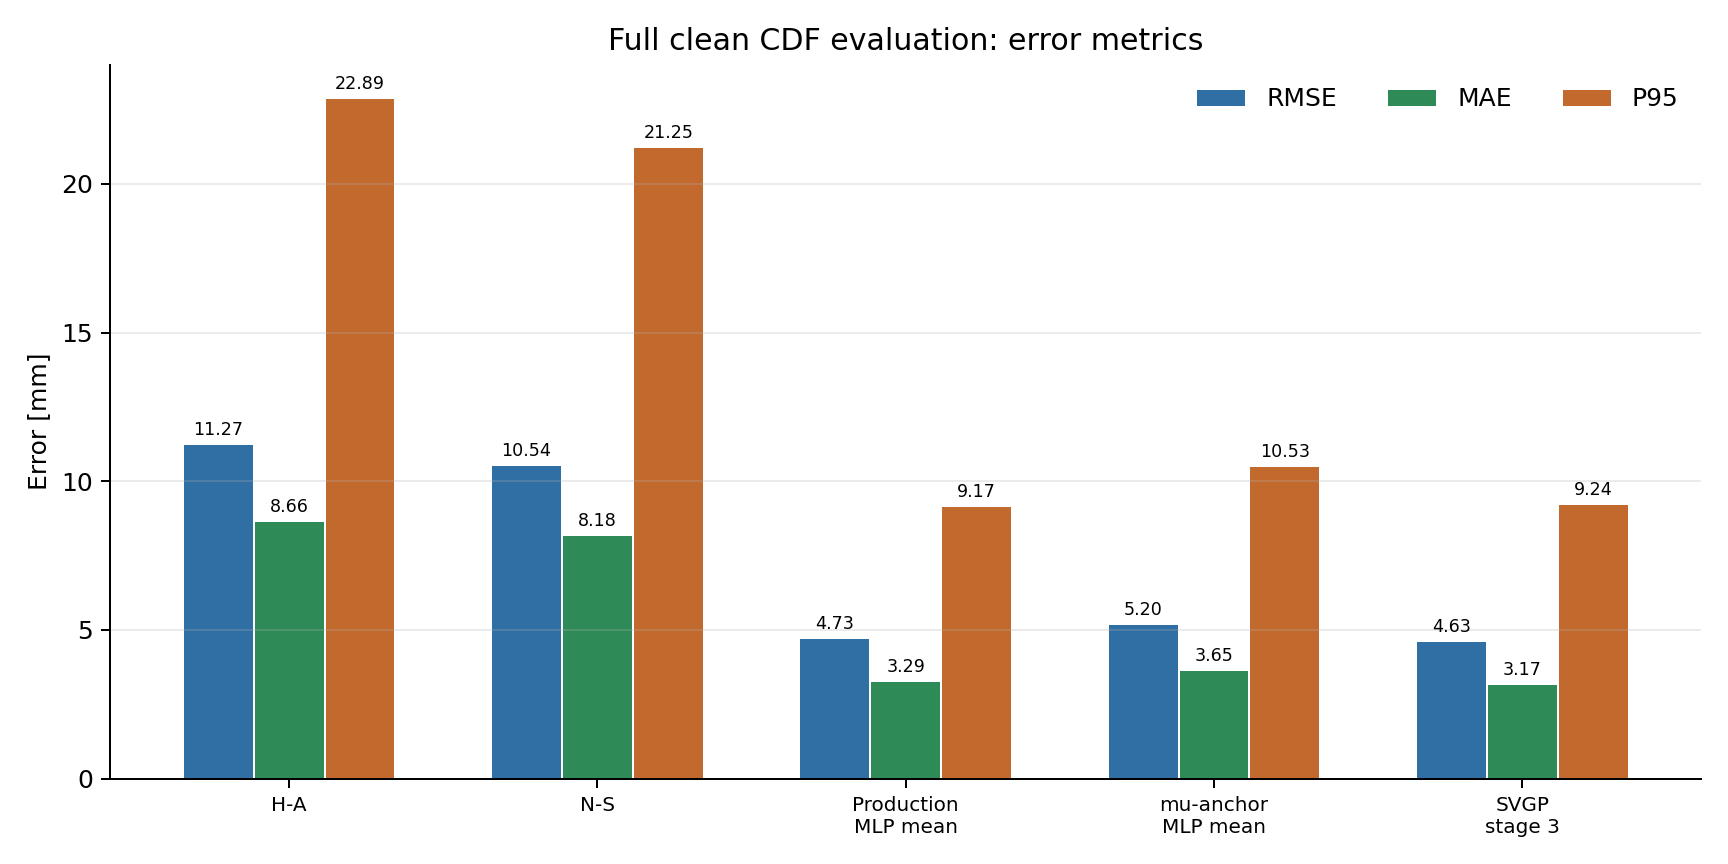
\includegraphics[width=0.92\linewidth,height=0.74\textheight,keepaspectratio]{full_clean_metric_bars_rmse_mae_p95.png}
\src{Thesis/images/baseline_comparison_20260521/full_clean_metric_bars_rmse_mae_p95.png}
\end{frame}

\begin{frame}{Full-Clean: Coverage}
\centering
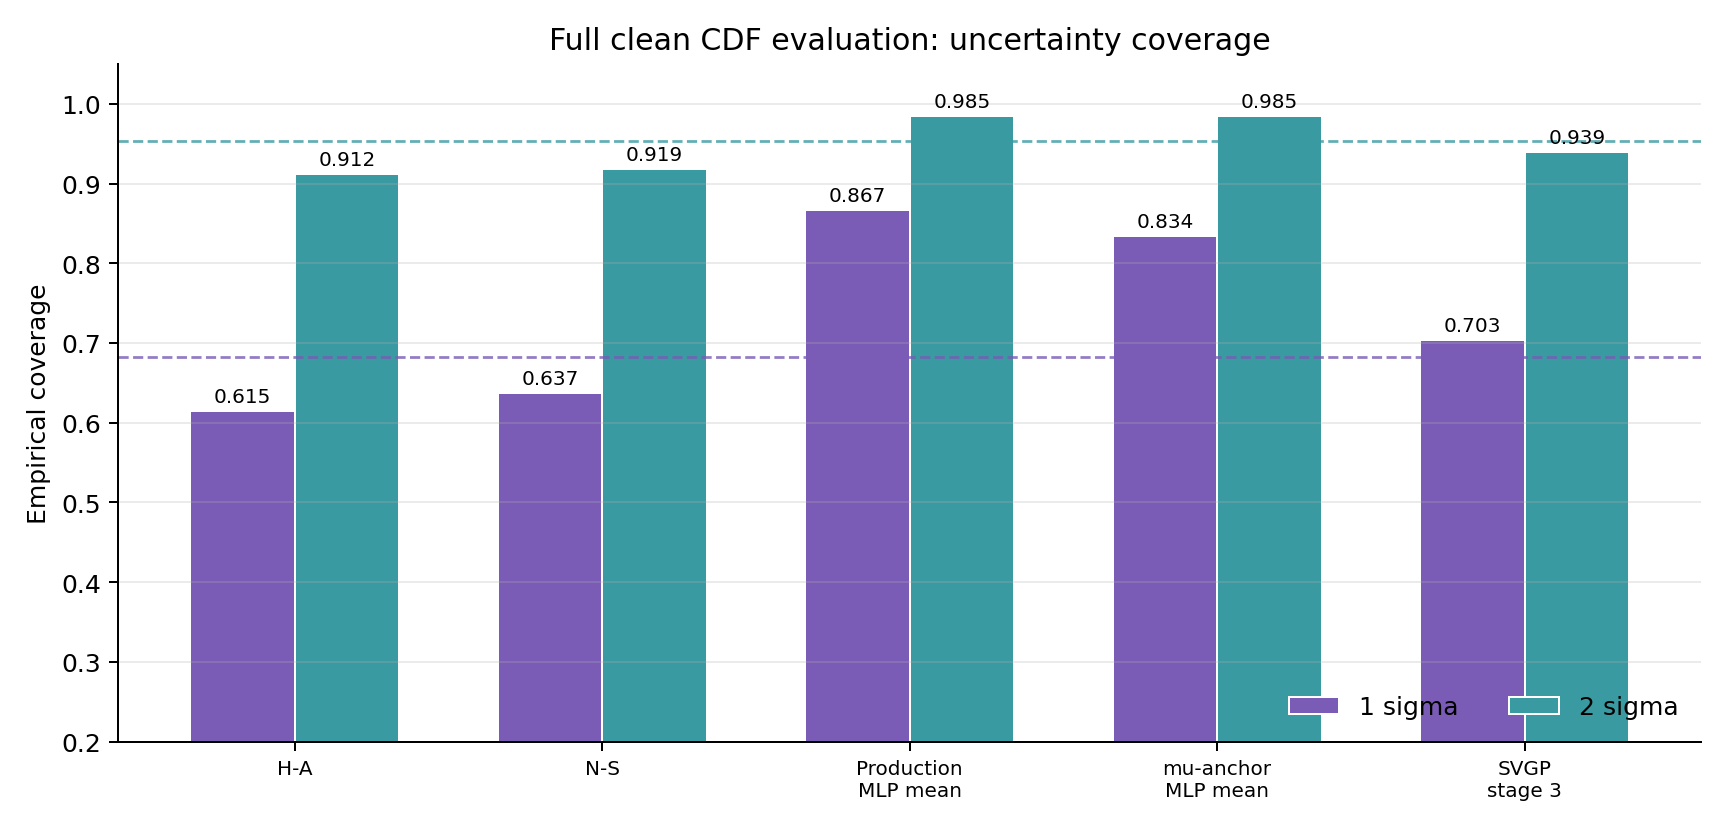
\includegraphics[width=0.88\linewidth,height=0.74\textheight,keepaspectratio]{full_clean_coverage_comparison.png}
\src{Thesis/images/baseline_comparison_20260521/full_clean_coverage_comparison.png}
\end{frame}

\begin{frame}{Production MLP Five-Seed Stability}
\begin{columns}[T,onlytextwidth]
\begin{column}{0.58\linewidth}
\centering
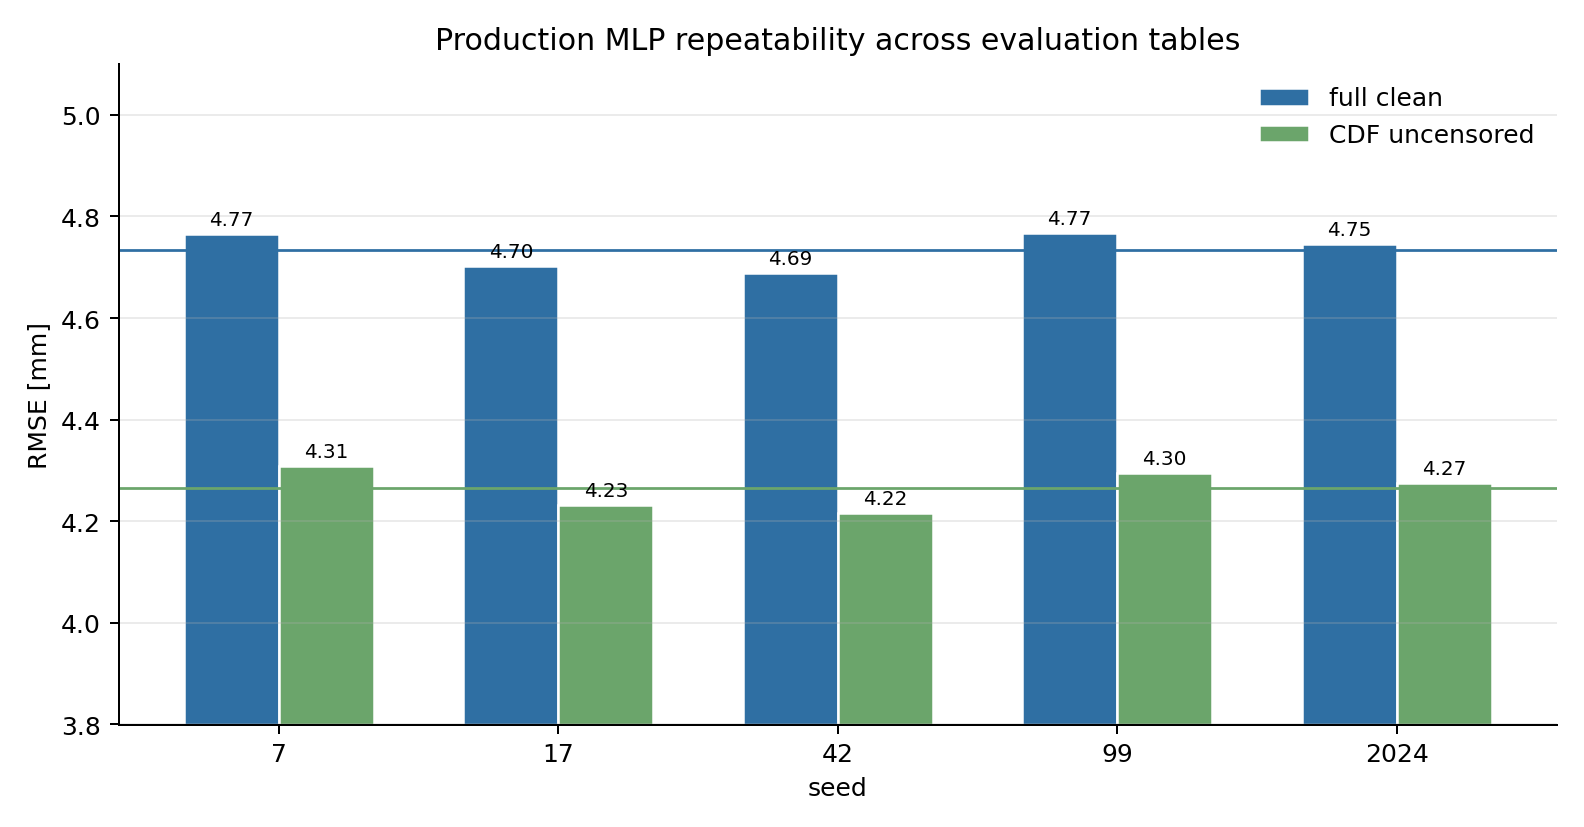
\includegraphics[width=\linewidth,height=0.70\textheight,keepaspectratio]{production_mlp_per_seed_rmse.png}
\end{column}
\begin{column}{0.38\linewidth}
\small
\begin{block}{Full-clean aggregate}
\begin{itemize}
  \item RMSE \(= \SI{4.735}{mm} \pm \SI{0.037}{mm}\)
  \item MAE \(= \SI{3.293}{mm} \pm \SI{0.039}{mm}\)
  \item Bias \(= +\SI{0.626}{mm} \pm \SI{0.112}{mm}\)
  \item Cov1/Cov2 \(= 0.867 / 0.985\)
\end{itemize}
\end{block}
\begin{block}{Reading}
\footnotesize
This is not seed luck: the five-seed RMSE spread is only about \SI{0.04}{mm}.
\end{block}
\end{column}
\end{columns}
\src{Thesis/generated/baseline_comparison_20260521/production_mlp_full_clean_per_seed.csv}
\end{frame}

\begin{frame}{Conservative Uncensored CDF}
\scriptsize
\begin{tabular}{L{0.29\linewidth}R{0.10\linewidth}R{0.10\linewidth}R{0.10\linewidth}R{0.10\linewidth}R{0.10\linewidth}R{0.10\linewidth}}
\toprule
Model & RMSE & MAE & Bias & P95 & Cov1 & Cov2 \\
\midrule
Hiroyasu--Arai & 10.261 & 7.767 & +2.152 & 21.095 & 0.630 & 0.917 \\
Naber--Siebers & 9.286 & 7.195 & +0.628 & 18.408 & 0.659 & 0.927 \\
\good{Production MLP mean(5)} & \good{4.265} & \good{3.032} & +0.562 & \good{8.307} & \good{0.887} & \good{0.989} \\
mu-anchor raw-uncertain & 4.941 & 3.505 & -0.868 & 10.123 & 0.840 & 0.988 \\
\blue{SVGP Stage-3} & \blue{4.193} & \blue{2.894} & -0.040 & 8.461 & 0.716 & 0.945 \\
\bottomrule
\end{tabular}

\vspace{0.6em}
\small
After conservative censoring control, production MLP and SVGP remain close:
SVGP has slightly lower RMSE, while MLP keeps wider coverage.
\src{Thesis/generated/baseline_comparison_20260521/fixed_table_group_summary.csv}
\end{frame}

\begin{frame}{Uncensored CDF: Error and Coverage}
\begin{columns}[T,onlytextwidth]
\begin{column}{0.50\linewidth}
\centering
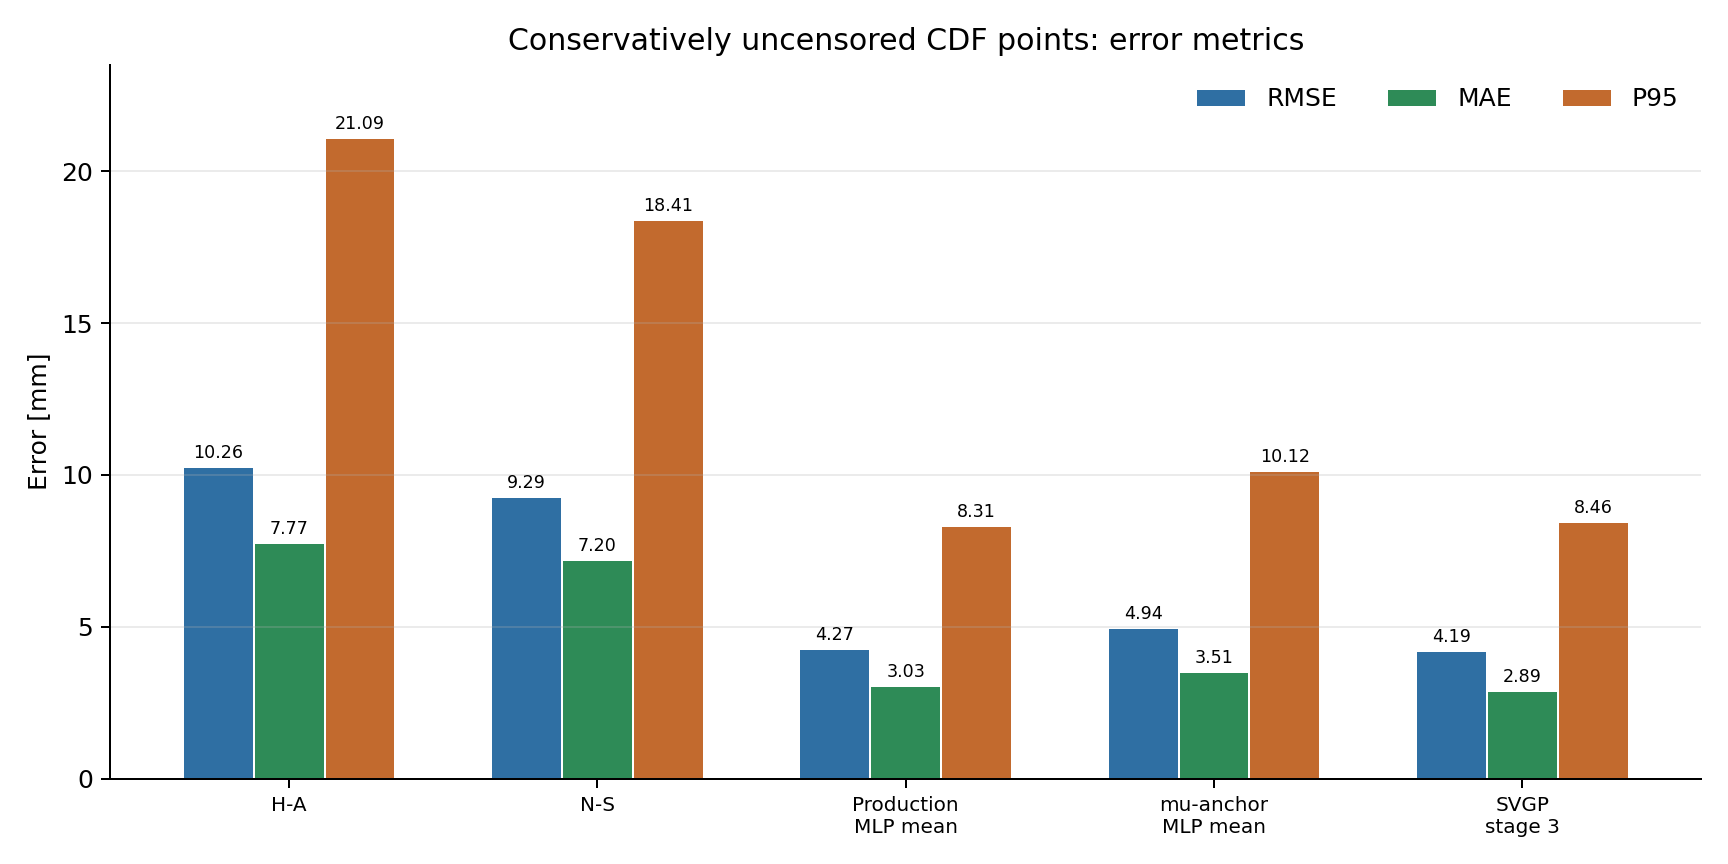
\includegraphics[width=\linewidth,height=0.70\textheight,keepaspectratio]{cdf_uncensored_metric_bars_rmse_mae_p95.png}
\end{column}
\begin{column}{0.50\linewidth}
\centering
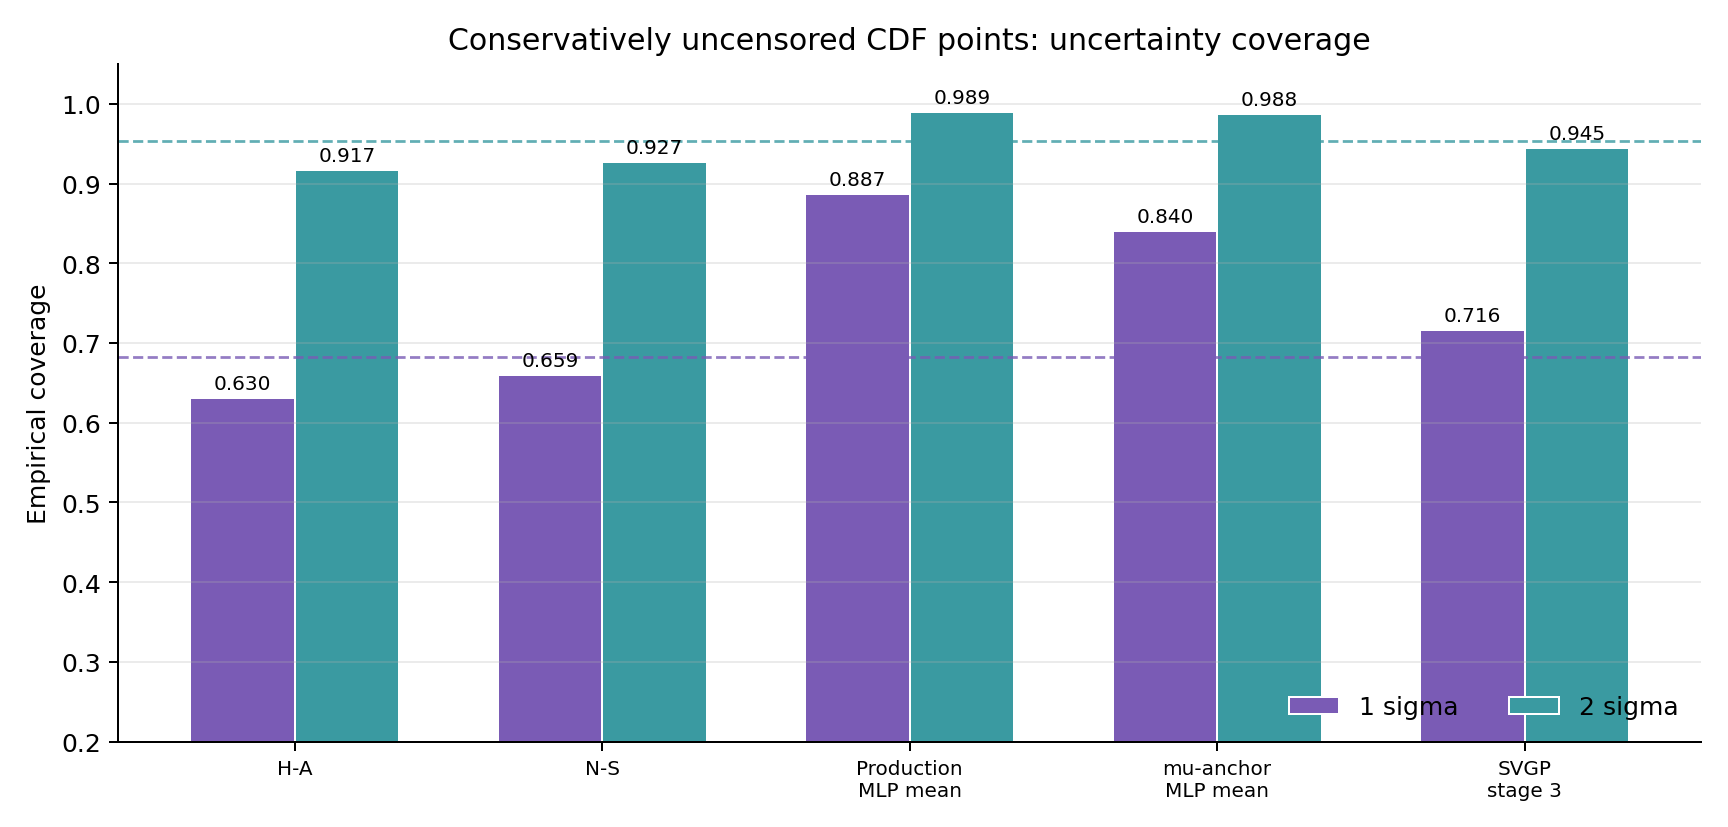
\includegraphics[width=\linewidth,height=0.70\textheight,keepaspectratio]{cdf_uncensored_coverage_comparison.png}
\end{column}
\end{columns}
\src{Thesis/images/baseline_comparison_20260521/cdf_uncensored_*.png}
\end{frame}

\begin{frame}{P50 and Q1 Protocols}
\scriptsize
\begin{tabular}{L{0.27\linewidth}R{0.13\linewidth}R{0.13\linewidth}R{0.13\linewidth}R{0.13\linewidth}}
\toprule
Model & P50 RMSE & P50 MAE & Q1 extrap. RMSE & Q1 extrap. MAE \\
\midrule
Q1 oracle & 1.010 & 0.689 & -- & -- \\
Hiroyasu--Arai & 9.948 & 7.662 & 31.837 & 25.316 \\
Naber--Siebers & 9.048 & 7.206 & 39.818 & 32.216 \\
\good{Production MLP mean(5)} & \good{2.848} & \good{1.826} & 10.864 & 7.380 \\
\good{mu-anchor raw-uncertain} & 3.212 & 2.147 & \good{10.358} & \good{6.965} \\
\blue{SVGP Stage-3} & \blue{2.649} & \blue{1.603} & 10.591 & 7.236 \\
\bottomrule
\end{tabular}

\vspace{0.6em}
\small
SVGP leads on P50 observed. The mu-anchor variant helps slightly on Q1
extrapolation, which is useful as a secondary result rather than the main
headline.
\src{Thesis/generated/baseline_comparison_20260521/fixed_table_group_summary.csv}
\end{frame}

\begin{frame}{P50 Observed and Q1 Extrapolated}
\begin{columns}[T,onlytextwidth]
\begin{column}{0.50\linewidth}
\centering
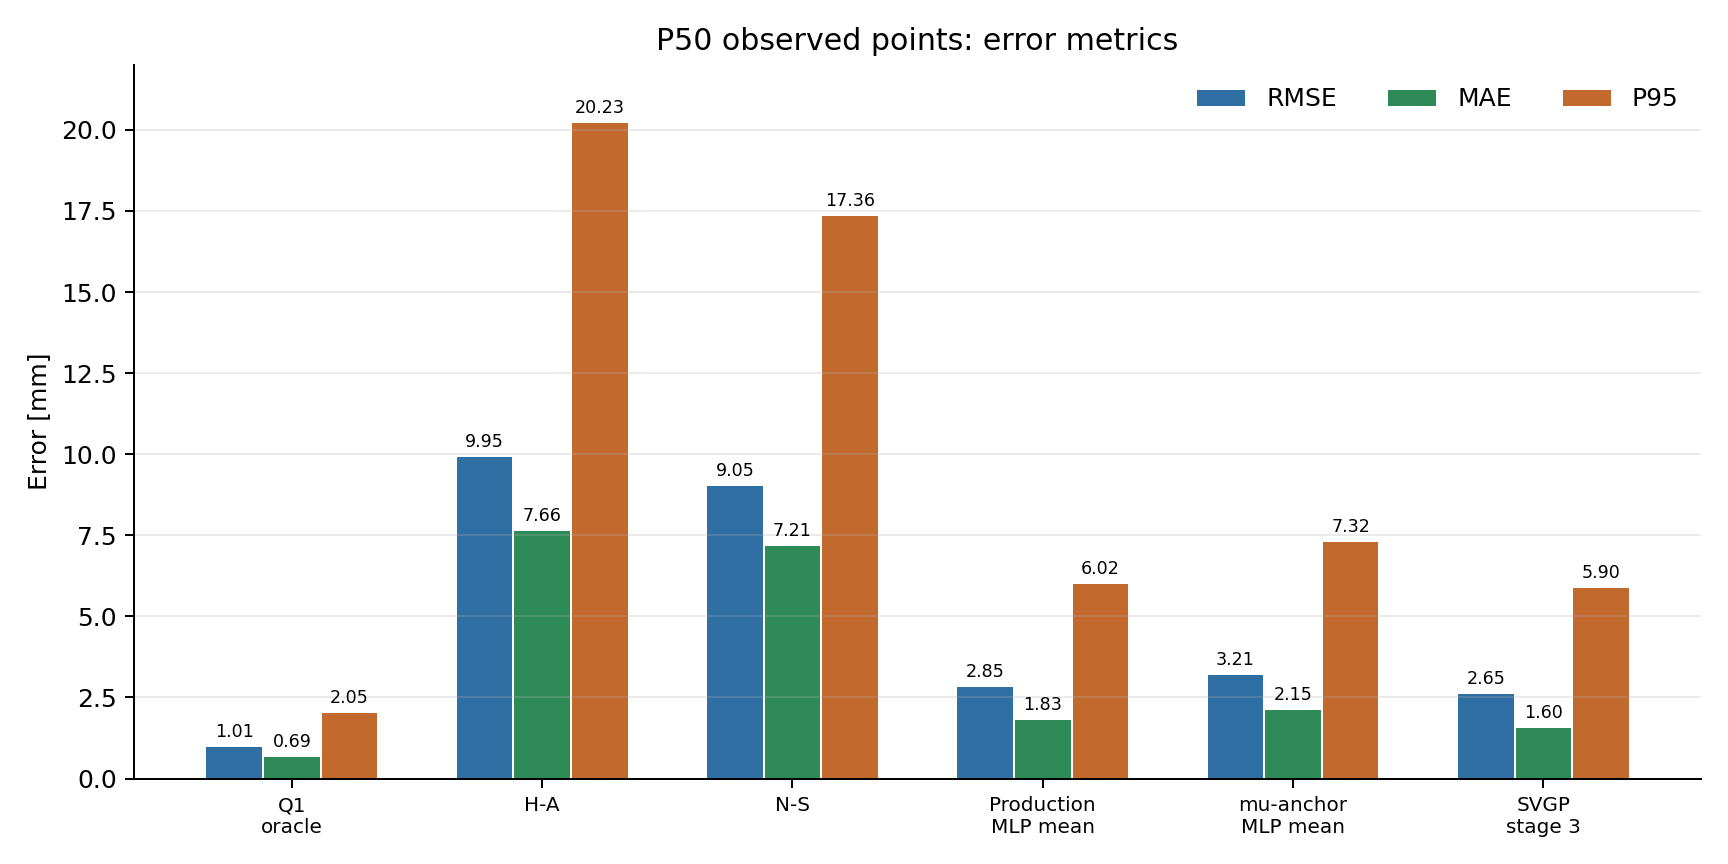
\includegraphics[width=\linewidth,height=0.70\textheight,keepaspectratio]{p50_observed_metric_bars_rmse_mae_p95.png}
\end{column}
\begin{column}{0.50\linewidth}
\centering
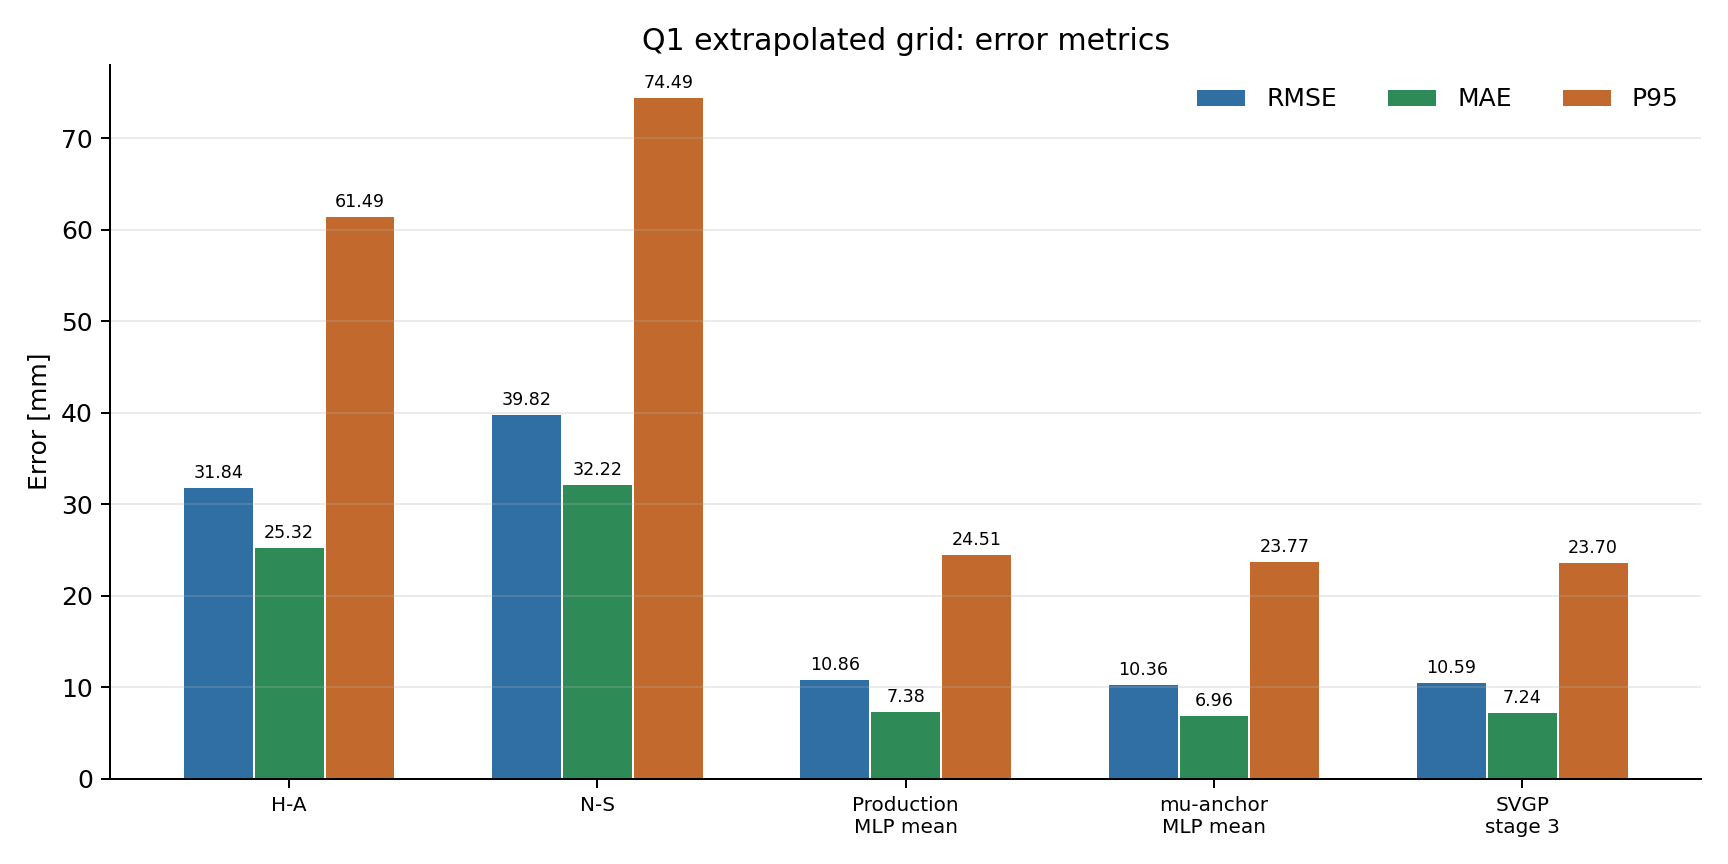
\includegraphics[width=\linewidth,height=0.70\textheight,keepaspectratio]{q1_extrapolated_metric_bars_rmse_mae_p95.png}
\end{column}
\end{columns}
\src{Thesis/images/baseline_comparison_20260521/p50_observed_*.png; q1_extrapolated_*.png}
\end{frame}

\begin{frame}{Thesis Narrative}
\small
\begin{enumerate}
  \item Do not claim that the MLP is ahead of SVGP; the latest results do not support that.
  \item Do claim that production MLP is far stronger than HA/NS on all clean, uncensored, and P50 protocols.
  \item Do report SVGP as the fair ML baseline and point-accuracy leader.
  \item Do emphasize that MLP uncertainty is more conservative and useful for downstream screening.
  \item Keep mu-anchor/raw-uncertain as a Q1 extrapolation supplement, not the main headline.
\end{enumerate}
\end{frame}

\begin{frame}{File Index}
\small
\begin{tabular}{L{0.30\linewidth}L{0.60\linewidth}}
\toprule
Item & Path \\
\midrule
Slides source & \pathtext{Thesis/slides/baseline_comparison_slides_en/baseline_comparison_slides_en.tex} \\
Figures & \pathtext{Thesis/images/baseline_comparison_20260521/} \\
Generated tables & \pathtext{Thesis/generated/baseline_comparison_20260521/} \\
Fixed-table report & \pathtext{MLP/baseline/comparison_reports/stage3_fixed_table_eval_with_ha_ns_20260521/} \\
Full-clean MLP vs SVGP & \pathtext{MLP/baseline/comparison_reports/mlp_production_stage3_vs_svgp_stage3_full_clean_20260521/} \\
Figure script & \pathtext{Thesis/generated/baseline_comparison_20260521/make_figures.py} \\
\bottomrule
\end{tabular}
\end{frame}

\end{document}
